% !TeX root = ../main.tex

\chapter{实验测试和分析}

基于上述章节,本章将对实现的ART索引进行相关的功能性测试和性能测试。
并且分析在有垃圾回收和无垃圾回收时内存使用情况。

\section{测试环境}

\subsection{硬件测试环境}
本次测试主要由一台主机完成,如下表所示其配置如下

% \usepackage{caption}

\begin{table}
\centering
\captionsetup{labelformat=empty}
\caption{服务器配置}
\begin{tabular}{|l|l|} 
\hline
cpu                  & ecs.c7a.8xlarge 32 vCPU       \\ 
\hline
内存                   & 64G      \\ 
\hline
硬盘                   & ESSD云盘 256GB  \\ 
\hline
操作系统                 & Ubuntu 20.04 (5.04.4)    \\ 
\hline
\multicolumn{1}{l}{} & \multicolumn{1}{l}{}    
\end{tabular}
\end{table}

\subsection{测试数据集和框架}
本次测试针对功能性测试主要测试索引插入,查询,范围查询,删除操作这些功能是否正确。
采取多种不同类型的数据(包括Int, Double,String)进行相关测试。除此之外,选取数据集时分别有顺序集合和随机集合。
依赖Google的GTest测试框架进行全面的测试。

\section{功能性测试}

针对功能性测试,主要测试索引操作算法的正确性,包括单线程,多线程操作的正确性,支持最长匹配的索引查询的正确性。

因此我们这里针对普通索引,使用Ints类型数据集和String类型数据集。根据插入顺序,生成1000万条数据。为了保证测试的
覆盖率。除了递增的数据之外,还需要对插入,查找随机数据集合。

\section{性能测试}
上述小节主要测试索引的功能性测试。本小节主要设计针对索引的性能测试。主要对比的是应用乐观级联锁之后,索引操作的可扩展
性是否达到预期要求。下面所有测试都是针对的并发读写的场景,考虑单一类型操作和读写混合操作。

\subsection{查询性能测试}

\begin{figure}[h]
  \centering
  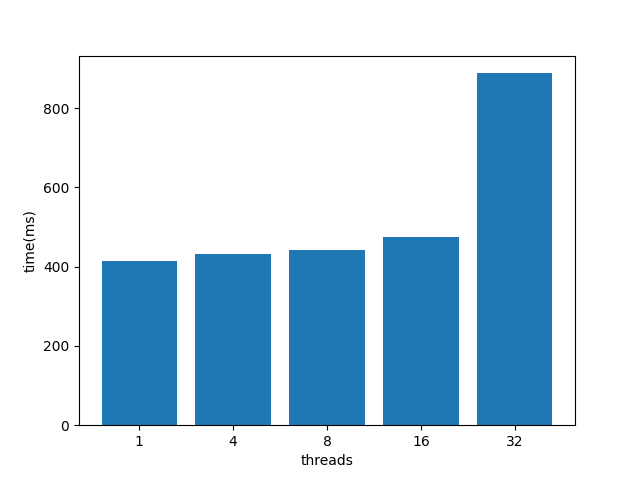
\includegraphics[width=0.9\textwidth]{lookup1.png}
  \caption{并发查询1000万条有序记录时间}
  \label{fig:cc-lookup-1}
\end{figure}

\begin{figure}[H]
  \centering
  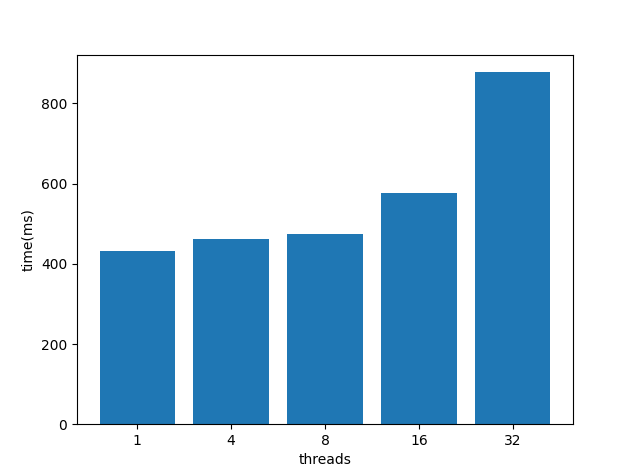
\includegraphics[width=0.9\textwidth]{lookup2.png}
  \caption{并发查询1000万条随机记录时间}
  \label{fig:cc-lookup-2}
\end{figure}

对于查询的性能测试,主要设计的数据集为1000万条,首先系统导入这1000万条数据,随后分别由1,4,8,16,32个线程进行查询测试
测试的结果如上图所示,以下表中包括顺序查询,随机点查询。

针对顺序数据的查询,1至16个工作线程分别查询1000万记录的耗时基本相同,但是32线程查询时,由于测试平台的核数仅有32个vCPU,这里导致线程调度的开销切换过大,
导致影响了正常的索引查询操作。造成一个突出的峰值。

针对随机数据的查询,综合上图的结果来看,与顺序查询的结果基本一致,即是乐观锁对于只读操作来说,多核扩展性较为友好。

\subsection{插入性能测试}

\begin{figure}[H]
  \centering
  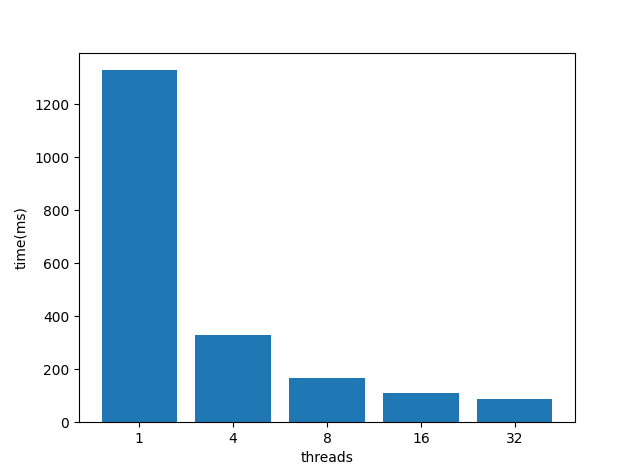
\includegraphics[width=0.9\textwidth]{insert1.png}
  \caption{并发插入1000万条有序记录时间}
  \label{fig:cc-insert-1}
\end{figure}

\begin{figure}[H]
  \centering
  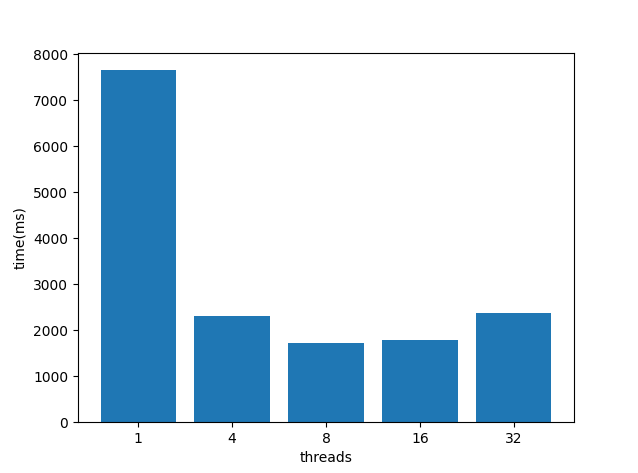
\includegraphics[width=0.9\textwidth]{insert2.png}
  \caption{并发插入1000万条随机记录时间}
  \label{fig:cc-insert-2}
\end{figure}


针对插入的性能测试,主要设计的数据集为1000万条,分别由1,4,8,16,32个线程进行插入测试,所有测试的总的数据记录的个数是相同的。即是最后
当所有线程操作完成之后,ART索引中都是只包含1000万条记录。
测试的结果如上图所示。

需要注意的是以下的插入数据分为两种。前者线程间插入的键值是互相离散的,即每个线程只负责插入某个区间的值,且区间和区间之间是完全不
重叠的,此时冲突较小。而后者我们可以看到同样是插入1000万条记录,对比同样的线程数,随机插入的吞吐量只有前者的十分之一。
这是因为当线程间插入随机数据时可能会频繁争用同一个索引内部节点时,导致冲突较大,在我么的索引实现中,采取的是当冲突增多之后的避让机制,这必然会导致线程挂起和睡眠。
因此多线程并行插入的效率就会产生较大的问题。

由此可以说明乐观锁的方式并不适合写冲突较高的场景,因为当写冲突较多操作会不断回到根节点,然后执行重做。如果当前的操作的深度
过大,则执行重做的开销较大,会造成系统性能抖动,因此乐观锁的并发控制确实不适合写冲突高的场景。

\subsection{删除性能测试}

删除的性能测试和以上插入测试类似,当删除操作需要删除的数据记录之间重叠较多,并行删除的效率会大大降低。由此得出的结论与并发插入
时是一致的。就是基于乐观锁的ART索引并不适合作为需要被频繁修改的索引结构。

\begin{figure}[H]
  \centering
  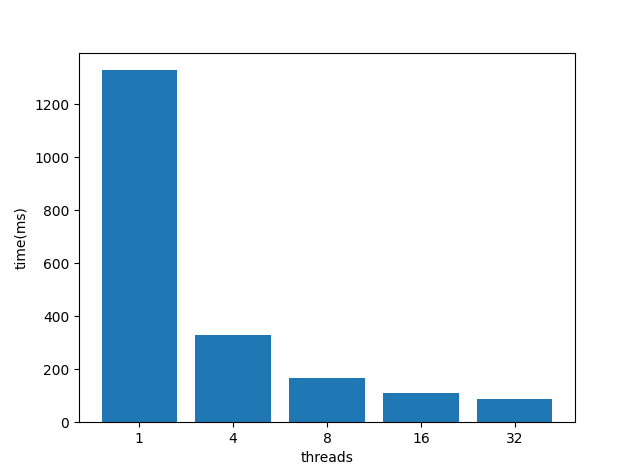
\includegraphics[width=0.9\textwidth]{delete1.png}
  \caption{并发删除1000万条有序记录时间}
  \label{fig:cc-delete-1}
\end{figure}

\begin{figure}[H]
  \centering
  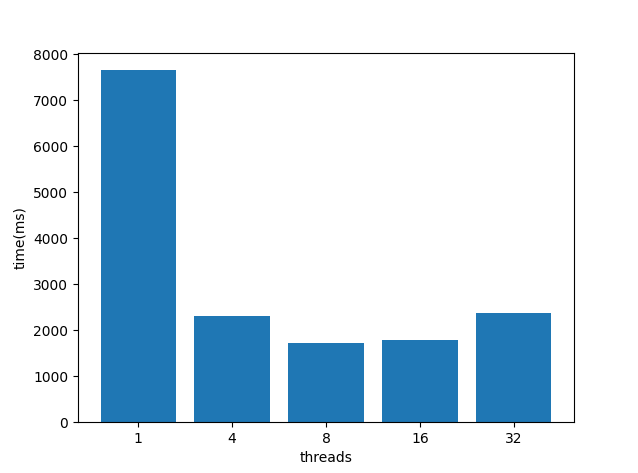
\includegraphics[width=0.9\textwidth]{delete2.png}
  \caption{并发删除1000万条随机记录时间}
  \label{fig:cc-delete-2}
\end{figure}

这里删除的性能测试结果与插入较为类似,也是一开始随着工作线程增多而获得较大的性能提升,但是随着工作线程的继续增加,所获得的
提升越小,甚至产生了副作用。

\subsection{查询/插入性能测试}

上述的测试中,只是针对单一的类型的负载进行测试,但是在实际应用中,并不存在只读或者只写类型的负载。
因此我们还设计了读写并行的测试数据。

\begin{figure}[H]
  \centering
  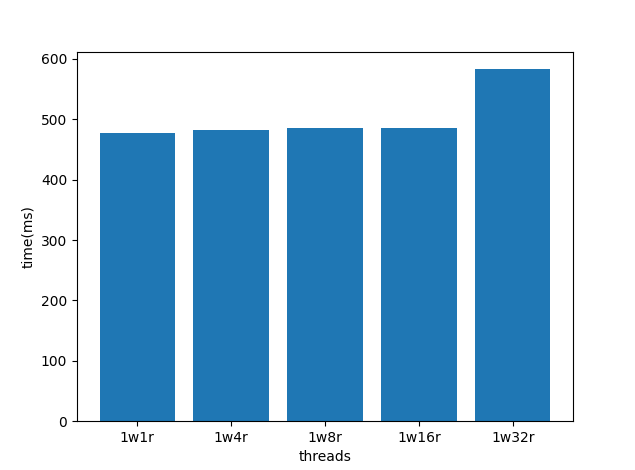
\includegraphics[width=0.9\textwidth]{rw.png}
  \caption{一写多读负载下的总耗时}
  \label{fig:rw}
\end{figure}

对于查询和插入的并行测试,主要是测试实际使用场景下多读单写情况,如下图所示,工作线程分为读线程和写线程,
分别为1写1读,1写4读,1写8读,1写16读,1写32读。测试其在并发情况下的性能,图中表明,随着并发线程的个数增长,完成所有操作需要的
时间并没有明显上升。表明基于乐观级联锁的ART索引在多核多线程使用场景下具备扩展性,基本满足设计预期。


\section{内存开销测试}

\begin{figure}[H]
  \centering
  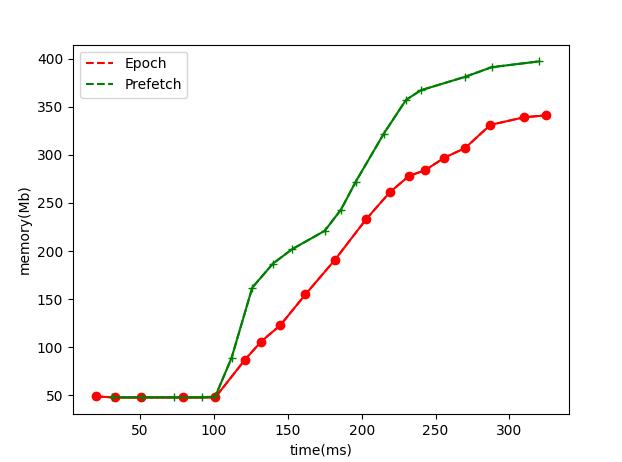
\includegraphics[width=0.9\textwidth]{memory.png}
  \caption{内存开销统计}
  \label{fig:memory}
\end{figure}


内存开销测试主要是针对不同数据量下,内存使用的开销,主要测试目的除了实际内存占用外,还需要测试在基于epoche的垃圾回收机制
对索引性能的影响。最终我们在多个数据量下进行测试,分别对比开启垃圾回收和不开启垃圾回收的吞吐量和内存开销。根据下图所示,在小数据量下
使用基于epoch的垃圾回收的效果较使用无锁队列收集删除节点差,但是在大数据量下,尤其是接近系统的上限时,由于此时操作系统内存较多
导致此时索引速度明显降低。因此我们在索引中设置一个阈值,超过阈值才会启动基于epoch的垃圾回收机制。这样两者结合可以获得较大的性能提升。

\section{本章小结}

本章主要介绍前文中设计和实现的基于乐观级联锁的索引及其相关模块的测试,第一小节介绍实际测试的环境,第二节针对前文中提到的相关
功能进行功能测试,第三节中主要进行相关性能测试,主要测试目的在于测试该索引在性能上是否达到所预期的效果,尤其是在多读少写的场景下
是否达到预期的效果。综合上述的测试也可以说明基于乐观锁的ART并不适合频繁修改的场景。

由上可见,在合适的使用场景下选择合适的数据结构,而且没有任何一种结构,可以适用于任何场景。此外经过系统的测试,可以发现在工程上
可以作出适当的取舍,融合两种不同的内存分配模式,获得最佳的效果。